% !Mode:: "TeX:UTF-8"
% !TEX program  = xelatex

%\documentclass{cumcmthesis}
\documentclass[withoutpreface,bwprint]{cumcmthesis} %去掉封面与编号页

\usepackage{url}   % 网页链接
\usepackage{cases}
\usepackage{subcaption} % 子标题
\title{全国大学生数学建模竞赛编写的 \LaTeX{} 模板}
\tihao{A}
\baominghao{4321}
\schoolname{XX大学}
\membera{}
\memberb{向左}
\memberc{哈哈}
\supervisor{老师}
\yearinput{2017}
\monthinput{08}
\dayinput{22}

\title{二维非齐次热传导方程的向后Crank-Nicolson ADI格式}
\begin{document}
	\maketitle
	~\\
	~\\
	
	作业:
	
	$$
	\left\{
	\begin{array}{lcl}
	\dfrac{\partial{u}}{\partial{t}}-(\dfrac{\partial^{2}{u}}{\partial{x}^{2}}+\dfrac{\partial^{2}{u}}{\partial{y}^{2}})=- \dfrac{3}{2}e^{\frac{1}{2}(x+y)-t} &,&0 < x,y < 1,0 < t \leq 1 \\
	
	u(x,y,0)=e^{\frac{1}{2}x-t} &, & 0 < x,y < 1 \\
	
	u(0,y,t)=e^{\frac{1}{2}y-t},u(1,y,t)=e^{\frac{1}{2}(1+y)-t},&, &0 \leq y \leq 1,0 \leq t \leq 1 \\
	
	u(x,0,t)=e^{\frac{1}{2}x-t},u(x,1,t)=e^{\frac{1}{2}(1+x)-t},&, &0 < x < 1,0 \leq t \leq 1 
	\end{array}
	\right.
	$$

该问题的精确解为$ u(x,y,t)=e^{\frac{1}{2}(x+y)-t}$.

定义误差为$$ E_{\infty}(h,\tau)=\max \limits_{1 \leq i,j \leq m-1 \atop 1 \leq k \leq n } |u_{i,j}^k-u(x_i,y_j,t_k)| $$

用向后Crank-Nicolson ADI格式求下述问题的数值解并对数值解、精度和误差阶进行相应的数值分析。


~\\
~\\

解:

将x和y  m等分,将t  n等分, 记$h=\dfrac{1}{m},\tau=\dfrac{1}{n}$

$x_i=ih,0 \leq i \leq m$
$y_j=jh,0 \leq j \leq m$
$t_k=k \tau,0 \leq k \leq n$


令$\gamma=\dfrac{\tau}{h^2}$

P-R差分格式为
%\begin{subequations}
%\begin{numcases}{}
%	3x+4y=5\\
%	5x-9y=13
%\end{numcases}
%\end{subequations}

\begin{subequations}
	\begin{numcases}{}
		(I-\dfrac{\tau}{2} \delta_x^2) \overline{u_{i,j}}=(I+\dfrac{\tau}{2} \delta_y^2)u_{i,j}^{k}+\dfrac{\tau}{2} f_{i,j}^{k+\frac{1}{2}} ,1 \leq i \leq m-1 \\
		(I-\dfrac{\tau}{2} \delta_y^2) u_{i,j}^{k+1}=(I+\dfrac{\tau}{2} \delta_x^2)\overline{u_{i,j}}+\dfrac{\tau}{2} f_{i,j}^{k+\frac{1}{2}} ,1 \leq j \leq m-1 
	\end{numcases}
\end{subequations}

其中
$Iu_{i,j}^k=u_{i,j}^k$,$\overline{u_{i,j}}$为中间层。
$\delta_x^2u_{i,j}=\dfrac{u_{i+1,j}-2u_{i,j}+u_{i-1,j}}{h^2}.$

$\delta_y^2u_{i,j}=\dfrac{u_{i,j+1}-2u_{i,j}+u_{i,j-1}}{h^2}.$

中间层的初值为
\begin{subequations}
	\begin{numcases}{}
	\overline{u_{0,j}}=\dfrac{1}{2}(u_{0,j}^{k}+u_{0,j}^{k+1})-\dfrac{\tau}{4}(\delta_y^2 u_{0,j}^{k+1}-\delta_y^2 u_{0,j}^{k}) \\
	\overline{u_{m,j}}=\dfrac{1}{2}(u_{m,j}^{k}+u_{m,j}^{k+1})-\dfrac{\tau}{4}(\delta_y^2 u_{m,j}^{k+1}-\delta_y^2 u_{m,j}^{k}) 
	\end{numcases}
\end{subequations}

(1a)可以写成矩阵形式

$$A \overline{u_{i,j}}=B_1^{k+1}$$.

$$
A=
\begin{bmatrix}
	1+\gamma & -\dfrac{\gamma}{2} \\
	-\dfrac{\gamma}{2} & 1+\gamma & -\dfrac{\gamma}{2} \\
	& \ddots & \ddots & \ddots \\
	& & 	-\dfrac{\gamma}{2} & 1+\gamma
\end{bmatrix}
$$

$$
B_1^{k+1}=
\dfrac{\gamma}{2}\cdot
\begin{bmatrix}
	u_{1,j-1}^{k-1} \\
	u_{2,j-1}^{k-1} \\
	\vdots \\
	u_{m-1,j-1}^{k-1} \\
\end{bmatrix}
+(1-\gamma) \cdot
\begin{bmatrix}
u_{1,j}^{k-1} \\
u_{2,j}^{k-1} \\
\vdots \\
u_{m-1,j}^{k-1} \\
\end{bmatrix}
+\dfrac{\gamma}{2}\cdot
\begin{bmatrix}
u_{1,j+1}^{k-1} \\
u_{2,j+1}^{k-1} \\
\vdots \\
u_{m-1,j+1}^{k-1} \\
\end{bmatrix}
+\dfrac{\tau}{2} \cdot
\begin{bmatrix}
f_{1,j}^{k+\frac{1}{2}}\\
f_{2,j}^{k+\frac{1}{2}}\\
\vdots \\
f_{m-1,j}^{k+\frac{1}{2}}\\
\end{bmatrix}
$$

(1b)可写成矩阵形式

$$A u_{i,j}^{k+1}=B_2^{k+1}$$.

$$
B_2^{k+1}=
\dfrac{\gamma}{2}\cdot
\begin{bmatrix}
\overline{u_{i-1,1}} \\
\overline{u_{i-1,2}} \\
\vdots \\
\overline{u_{i-1,m-1}} \\
\end{bmatrix}
+(1-\gamma) \cdot
\begin{bmatrix}
\overline{u_{i,1}} \\
\overline{u_{i,2}} \\
\vdots \\
\overline{u_{i,m-1}} \\
\end{bmatrix}
+\dfrac{\gamma}{2}\cdot
\begin{bmatrix}
\overline{u_{i+1,1}} \\
\overline{u_{i+1,2}} \\
\vdots \\
\overline{u_{i+1,m-1}} \\
\end{bmatrix}
+\dfrac{\tau}{2} \cdot
\begin{bmatrix}
f_{i,1}^{k+\frac{1}{2}}\\
f_{i,2}^{k+\frac{1}{2}}\\
\vdots \\
f_{i,m-1}^{k+\frac{1}{2}}\\
\end{bmatrix}
$$
两个方程的系数矩阵均为三对角矩阵。
~\\
~\\




\textbf{解题程序运行于Matlab 2018a}

$\tau=\dfrac{1}{10},h=\dfrac{1}{10}$时t=1处的数值解和精确解见图\ref{fig:f1},非常接近。
\begin{figure}
	\centering
	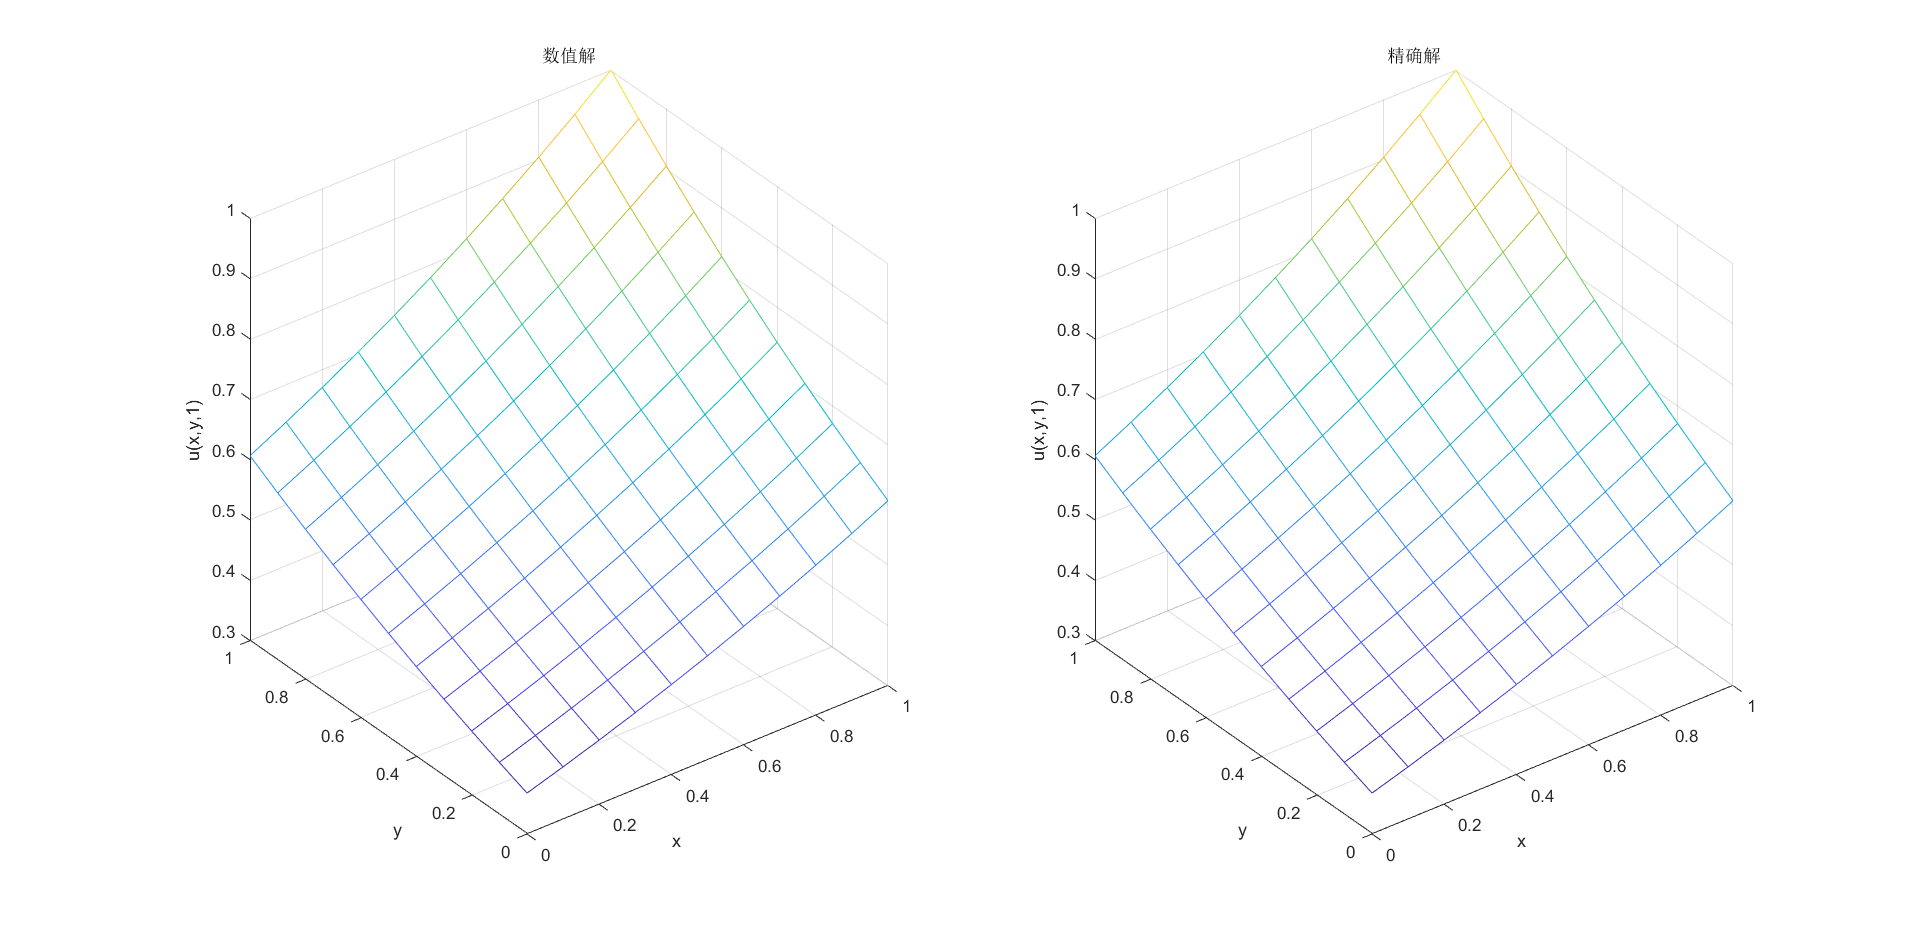
\includegraphics[width=1\linewidth]{figures/f1}
	\caption{$\tau=\dfrac{1}{10},h=\dfrac{1}{10}$时t=1处的数值解和精确解}
	\label{fig:f1}
\end{figure}

部分节点处的数值解、精确解和误差见表\ref{tab:1}.
\begin{table}[htbp]
	\centering
	\caption{部分节点处的数值解、精确解和误差}
	\begin{tabular}{cccc}
		\toprule[1.5pt]
		t,x,y & 数值解   & 精确解   & 误差 \\
		\midrule[1pt]
		0.1,0.5,0.5 & 1.491952  & 1.491825  & 1.2683E-04 \\
		0.2,0.5,0.5 & 1.349996  & 1.349859  & 1.3688E-04 \\
		0.3,0.5,0.5 & 1.221528  & 1.221403  & 1.2516E-04 \\
		0.4,0.5,0.5 & 1.105285  & 1.105171  & 1.1366E-04 \\
		0.5,0.5,0.5 & 1.000103  & 1.000000  & 1.0285E-04 \\
		0.6,0.5,0.5 & 0.904930  & 0.904837  & 9.3073E-05 \\
		0.7,0.5,0.5 & 0.818815  & 0.818731  & 8.4216E-05 \\
		0.8,0.5,0.5 & 0.740894  & 0.740818  & 7.6202E-05 \\
		0.9,0.5,0.5 & 0.670389  & 0.670320  & 6.8951E-05 \\
		1.0,0.5,0.5 & 0.606593  & 0.606531  & 6.2389E-05 \\
		\bottomrule[1.5pt]
	\end{tabular}%
	\label{tab:1}%
\end{table}%


t=1时,取不同步长时的误差见图\ref{fig:2},步长越小,误差越小。
\begin{figure*}
	\centering
	\begin{subfigure}[b]{0.475\textwidth}
		\centering
		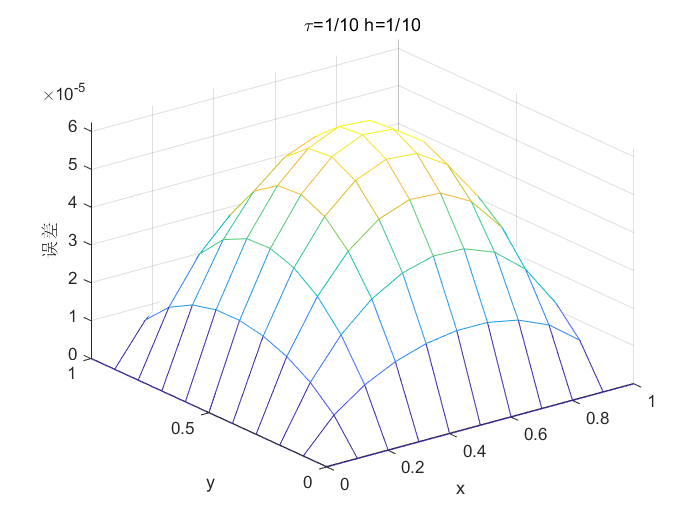
\includegraphics[width=\textwidth]{figures/f2}
		\caption[Network2]%
		{{\small $h=1/10,\tau=1/10$时的误差}}    
		\label{fig:mean and std of net14}
	\end{subfigure}
	\hfill
	\begin{subfigure}[b]{0.475\textwidth}  
		\centering 
		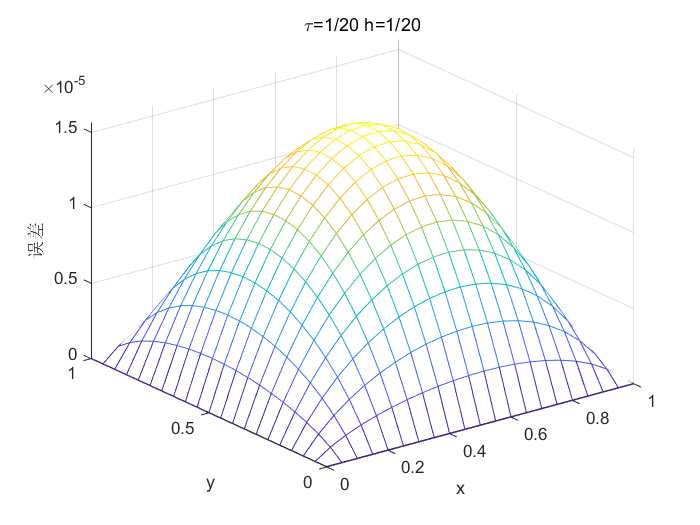
\includegraphics[width=\textwidth]{figures/f3}
		\caption[]%
		{{\small $h=1/20,\tau=1/20$时的误差}}    
		\label{fig:mean and std of net24}
	\end{subfigure}
	\vskip\baselineskip
	\begin{subfigure}[b]{0.475\textwidth}   
		\centering 
		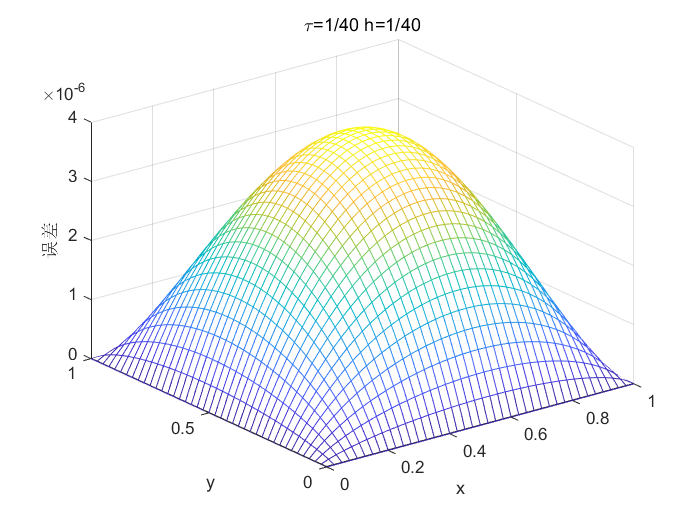
\includegraphics[width=\textwidth]{figures/f4}
		\caption[]%
		{{\small $h=1/40,\tau=1/40$时的误差}}    
		\label{fig:mean and std of net34}
	\end{subfigure}
	\quad
	\begin{subfigure}[b]{0.475\textwidth}   
		\centering 
		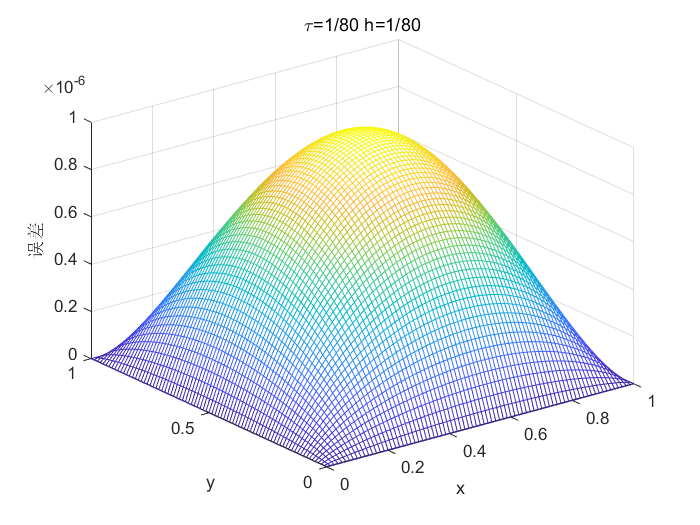
\includegraphics[width=\textwidth]{figures/f5}
		\caption[]%
		{{\small $h=1/180,\tau=1/80$时的误差}}    
		\label{fig:mean and std of net44}
	\end{subfigure}
	\caption[ The average and standard deviation of critical parameters ]
	{t=1时的误差图} 
	\label{fig:2}
\end{figure*}
	
	取不同步长时的最大误差和最大误差的比见表\ref{tab:2},$h$变为原来的
	2倍,$\tau$变为原来的2倍,最大误差变为原来的4倍,符合$O(\tau^2+h^2)$的截断误差。
	% Table generated by Excel2LaTeX from sheet 'Sheet1'
	\begin{table}[htbp]
		\centering
		\caption{不同步长时的最大误差和最大误差的比}
		\begin{tabular}{ccc}
			\toprule[1.5pt]
			$h,\tau$   & $E_{\infty}(h,\tau)$ & $E_{\infty}(2h,2\tau)/E_{\infty}(h,\tau)$ \\
			\midrule[1pt]
			1/10,1/10 & 1.37E-04 & * \\
			1/20,1/20 & 3.44E-05 & 3.9795  \\
			1/40,1/40 & 8.57E-06 & 4.0113  \\
			1/80,1/80 & 2.15E-06 & 3.9937  \\
			\bottomrule[1.5pt]
		\end{tabular}%
		\label{tab:2}%
	\end{table}%
	

\end{document}